\chapter{Partie électronique}

\section{Schéma électrique}
\begin{figure}[H]
    \centering
    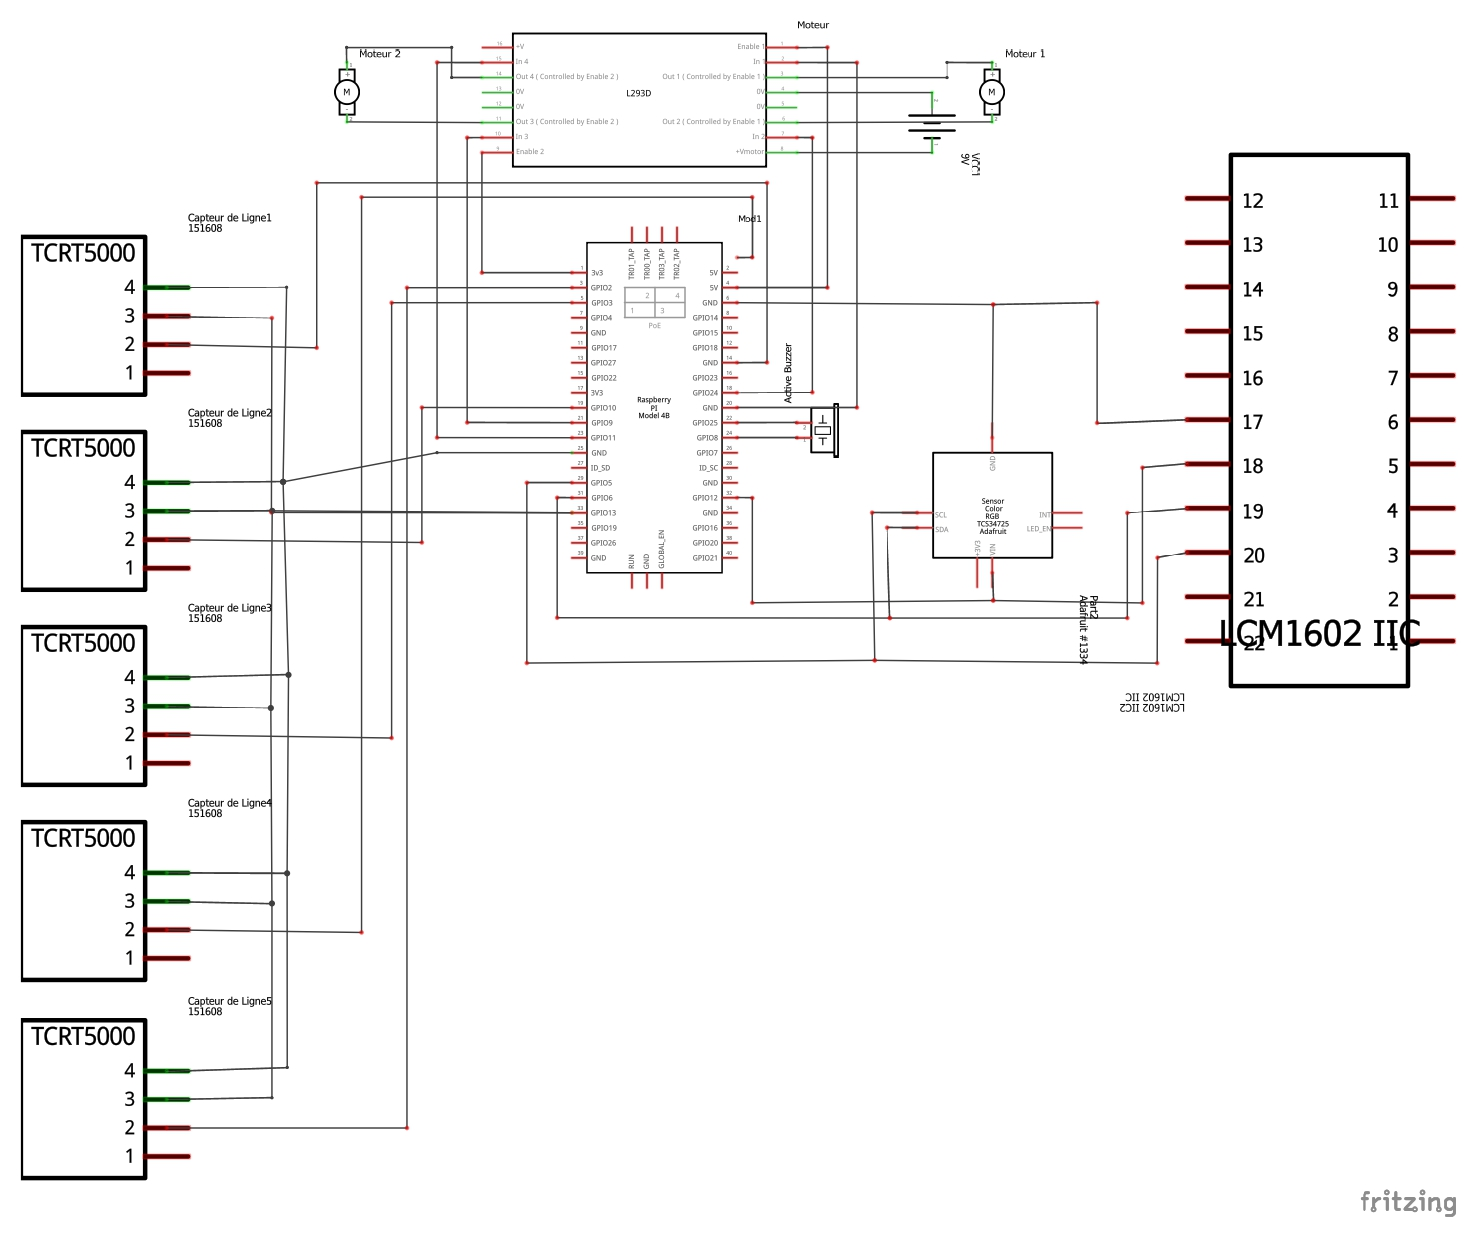
\includegraphics[width=0.9\textwidth]{parties/schema_electrique.jpg}
    \caption{Schéma électrique complet du robot.}
\end{figure}
% Si vous voulez, vous pouvez rediriger ici vers le doc fritzing au lieu d'un ong
Le module I2C, sur la boîte est normalement branché à l'écran LCD, mais il n'est pas branché par lisibilité du schéma, et que notre module était déjà branché de notre côté.
%hadi---

\section{Architecture matérielle du robot}

\subsection{Raspberry Pi : cœur du système}

\subsubsection{Rôle}
Le Raspberry Pi constitue le cerveau du robot. Il assure les fonctions suivantes :
\begin{itemize}
    \item lecture des données provenant des capteurs,
    \item traitement des informations,
    \item commande des moteurs,
    \item communication avec l’écran LCD et le capteur de couleur.
\end{itemize}

\subsubsection{Connexions principales}
\begin{itemize}
    \item GPIO $\rightarrow$ capteurs de ligne TCRT5000,
    \item GPIO $\rightarrow$ driver de moteurs L293D,
    \item GPIO I2C (SDA, SCL) $\rightarrow$ écran LCD et capteur de couleur,
    \item GPIO $\rightarrow$ buzzer,
    \item Alimentation 5V et GND $\rightarrow$ ensemble des modules.
\end{itemize}

%-------------------------------------------------

\subsection{Capteurs de ligne TCRT5000 (x5)}

\subsubsection{Rôle}
Les capteurs TCRT5000 sont des capteurs infrarouges utilisés pour :
\begin{itemize}
    \item détecter une ligne noire sur un fond clair (suivi de ligne),
    \item déterminer la position de la ligne sous le robot.
\end{itemize}

Chaque capteur est composé :
\begin{itemize}
    \item d’une LED infrarouge émettrice,
    \item d’un phototransistor récepteur.
\end{itemize}

\subsubsection{Connexions}

Chaque capteur TCRT5000 est alimenté par le Raspberry Pi et connecté à un GPIO distinct afin de permettre une lecture indépendante de la position de la ligne.

\begin{itemize}
    \item \textbf{Capteur arrière gauche:}
    \begin{itemize}
        \item VCC $\rightarrow$ 3.3V du Raspberry Pi,
        \item GND $\rightarrow$ GND du Raspberry Pi,
        \item OUT $\rightarrow$ GPIO21.
    \end{itemize}

    \item \textbf{Capteur avant gauche  :}
    \begin{itemize}
        \item VCC $\rightarrow$ 3.3V du Raspberry Pi,
        \item GND $\rightarrow$ GND du Raspberry Pi,
        \item OUT $\rightarrow$ GPIO22.
    \end{itemize}

    \item \textbf{Capteur avant droit :}
    \begin{itemize}
        \item VCC $\rightarrow$ 3.3V du Raspberry Pi,
        \item GND $\rightarrow$ GND du Raspberry Pi,
        \item OUT $\rightarrow$ GPIO3.
    \end{itemize}

    \item \textbf{Capteur arrière droit:}
    \begin{itemize}
        \item VCC $\rightarrow$ 3.3V du Raspberry Pi,
        \item GND $\rightarrow$ GND du Raspberry Pi,
        \item OUT $\rightarrow$ GPIO27.
    \end{itemize}

    \item \textbf{Capteur central à l’avant :}
    \begin{itemize}
        \item VCC $\rightarrow$ 3.3V du Raspberry Pi,
        \item GND $\rightarrow$ GND du Raspberry Pi,
        \item OUT $\rightarrow$ GPIO6.
    \end{itemize}
\end{itemize}


Sur le schéma, chaque capteur est connecté à un GPIO différent afin de permettre au Raspberry Pi d’analyser précisément la position de la ligne et de corriger la trajectoire du robot.

\subsubsection{Justification du nombre de capteurs}
L’utilisation de cinq capteurs permet :
\begin{itemize}
    \item une meilleure précision de détection,
    \item la reconnaissance des virages,
    \item la gestion des intersections.
\end{itemize}
Voir la partie positionnement et câblage des capteurs pour plus d'informations.

%-------------------------------------------------

\subsection{L293D : driver de moteurs}

\subsubsection{Rôle}
Le L293D est un circuit intégré de type pont en H. Il permet :
\begin{itemize}
    \item au Raspberry Pi, délivrant un faible courant, de commander des moteurs DC nécessitant un courant plus élevé,
    \item de faire fonctionner les moteurs en rotation avant, arrière ou à l’arrêt.
\end{itemize}

\subsubsection{Connexions côté Raspberry Pi}
\begin{itemize}
    \item IN1, IN2 $\rightarrow$ GPIO23,GPIO24 (commande du sens du moteur 1),
    \item IN3, IN4 $\rightarrow$ GPIO27,GPIO17 (commande du sens du moteur 2),
    \item Enable 1 et Enable 2 $\rightarrow$ GPIO12,GPIO13 (activation et contrôle de la vitesse par PWM),
    \item GND $\rightarrow$ masse commune,
    \item Vcc1 $\rightarrow$ 5V (alimentation logique),
    \item Vcc2 $\rightarrow$ alimentation des moteurs (9~\text{V})

\end{itemize}

%-------------------------------------------------

\subsection{Moteurs DC}

\subsubsection{Rôle}
Les moteurs DC assurent le déplacement du robot, permettant les mouvements vers la gauche et la droite.

\subsubsection{Connexions}
\begin{itemize}
    \item OUT1 / OUT2 du L293D $\rightarrow$ moteur 1,
    \item OUT3 / OUT4 du L293D $\rightarrow$ moteur 2.
\end{itemize}

\subsubsection{Remarque importante}
Les moteurs ne sont pas connectés directement au Raspberry Pi. Ils sont impérativement commandés via le driver L293D afin de protéger le microcontrôleur et de fournir une puissance suffisante.

%-------------------------------------------------

\subsection{Alimentation des moteurs (pile 9V)}

\subsubsection{Rôle}
La pile 9V est utilisée pour :
\begin{itemize}
    \item alimenter exclusivement les moteurs,
    \item éviter de surcharger le Raspberry Pi.
\end{itemize}

\subsubsection{Connexions}
\begin{itemize}
    \item +9V $\rightarrow$ Vcc2 du L293D,
    \item $-$ $\rightarrow$ GND commun.
\end{itemize}

\subsubsection{Masse commune}
La masse de la pile, du Raspberry Pi et du L293D est commune. Cette configuration est indispensable pour garantir une référence électrique identique et assurer le bon fonctionnement des signaux de commande.

%-------------------------------------------------

\subsection{Capteur de couleur TCS34725}

\subsubsection{Rôle}
Le capteur TCS34725 permet :
\begin{itemize}
    \item la détection de la couleur d’un objet ou du sol,
    \item la fourniture des composantes RGB.
\end{itemize}

\subsubsection{Communication}
Le capteur communique avec le Raspberry Pi via le bus I2C.

\subsubsection{Connexions}
\begin{itemize}
    \item VCC $\rightarrow$ 3.3V,
    \item GND $\rightarrow$ GND,
    \item SDA $\rightarrow$ GPIO SDA du Raspberry Pi,
    \item SCL $\rightarrow$ GPIO SCL du Raspberry Pi,
\end{itemize}

\subsubsection{Avantage}
Le capteur partage le même bus I2C que l’écran LCD, ce qui permet de réduire le nombre de GPIO utilisés.

%-------------------------------------------------

\subsection{Écran LCD 16x2 avec interface I2C}

\subsubsection{Rôle}
L’écran LCD permet l’affichage des informations du robot telles que :
\begin{itemize}
    \item l’état du système,
    \item la couleur détectée,
    \item le mode de fonctionnement.
\end{itemize}

\subsubsection{Connexions}
\begin{itemize}
    \item VCC $\rightarrow$ 5V,
    \item GND $\rightarrow$ GND,
    \item SDA $\rightarrow$ GPIO SDA (I2C),
    \item SCL $\rightarrow$ GPIO SCL (I2C).
\end{itemize}

\subsubsection{Avantage de l’I2C}
L’interface I2C nécessite uniquement deux fils de données, ce qui permet d’économiser les GPIO du Raspberry Pi.

%-------------------------------------------------

\subsection{Buzzer actif}

\subsubsection{Rôle}
Le buzzer actif est utilisé pour émettre des signaux sonores lors :
\begin{itemize}
    \item du démarrage du robot,
    \item d’alertes,
    \item de la détection d’événements spécifiques.
\end{itemize}

\subsubsection{Connexions}
\begin{itemize}
    \item borne positive $\rightarrow$ GPIO18 du Raspberry Pi,
    \item borne négative $\rightarrow$ GND.
\end{itemize}

\subsubsection{Remarque}
Étant un buzzer actif, il ne nécessite pas de signal PWM. Un niveau logique haut (\texttt{HIGH}) appliqué au GPIO18 suffit pour produire un son.

% hadi-----
\section{Choix techniques et câblage}

Cette section présente les principaux choix techniques réalisés lors de la conception du système, ainsi que l’organisation du câblage. Les décisions prises visent à garantir un fonctionnement fiable du robot, une protection des composants électroniques et une facilité d’intégration des différents modules.

\subsubsection{Câblage des moteurs via le L293D}

Les moteurs à courant continu ne sont pas connectés directement au Raspberry Pi. En effet, les broches GPIO du Raspberry Pi ne peuvent fournir qu’un courant limité, insuffisant pour alimenter des moteurs DC.

L’utilisation du driver de moteurs L293D, basé sur une architecture de type pont en H, permet :
\begin{itemize}
    \item d’amplifier le courant délivré aux moteurs,
    \item de protéger le Raspberry Pi contre les surintensités,
    \item de contrôler le sens de rotation des moteurs (avant et arrière),
    \item de gérer la mise en marche et l’arrêt des moteurs.
\end{itemize}

Les broches d’entrée du L293D (IN1 à IN4) sont reliées aux GPIO du Raspberry Pi afin de commander le sens de rotation des moteurs, tandis que les broches \textit{Enable} permettent l’activation et, si nécessaire, le contrôle de la vitesse par modulation de largeur d’impulsion (PWM).

\subsubsection{Alimentation du Raspberry Pi et des autres composants}

Le Raspberry Pi est alimentée indépendamment des moteurs afin d’assurer une tension stable et d’éviter les perturbations liées aux appels de courant des actionneurs. Les composants électroniques tels que les capteurs, l’écran LCD et le buzzer sont alimentés par le Raspberry Pi via les lignes 5V et 3.3V.

Les moteurs DC sont alimentés par une source externe dédiée (pile 9V), fournissant une tension mesurée d’environ $8{,}27~\text{V}$, soit approximativement $9~\text{V}$. Cette séparation des alimentations permet de limiter les chutes de tension et d’améliorer la fiabilité du système.

L’ensemble des composants partage une masse commune (GND), condition indispensable pour assurer une référence électrique cohérente et garantir le bon fonctionnement des signaux de commande.

\subsubsection{Positionnement et câblage des capteurs}
\begin{figure}[H]
    \centering
    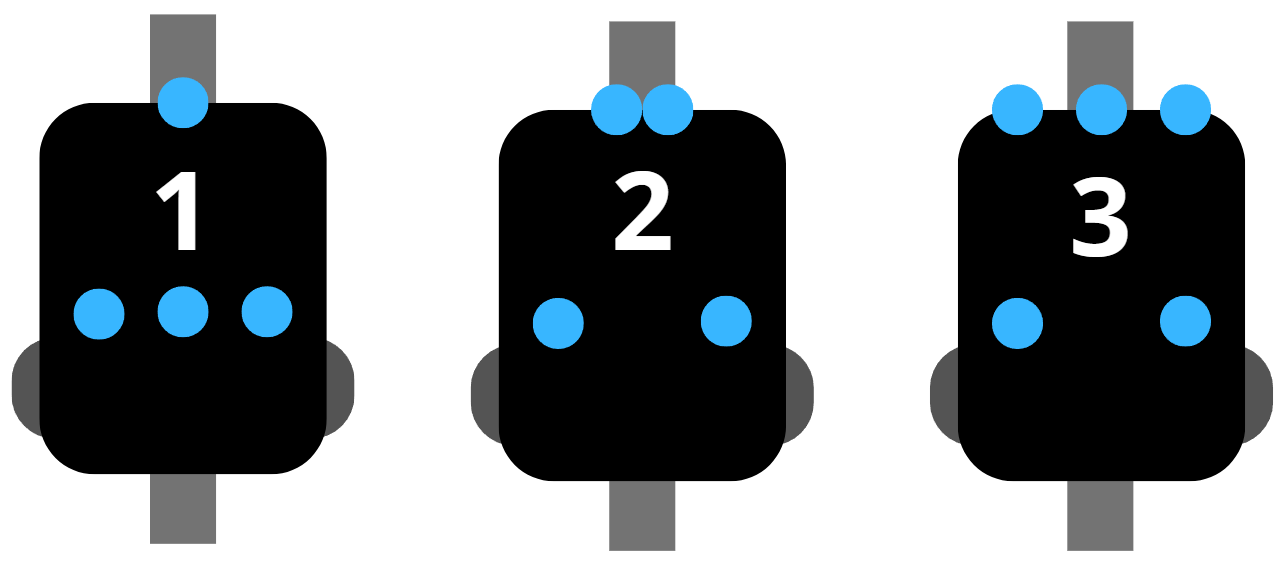
\includegraphics[width=0.9\textwidth]{images/disposition_capteurs.png}
    \caption{Différentes phases de conception et de disposition des capteurs}
\end{figure}

Les capteurs de ligne TCRT5000 sont positionnés à l’avant du robot afin de détecter la trajectoire à suivre. Leur disposition comprend un capteur central, des capteurs latéraux avant et des capteurs latéraux arrière, ce qui permet une détection précise de la ligne, y compris dans les virages et aux intersections. La figure 2.2 présente nos différentes phases de disposition de ces capteurs, ayant débuté par le 1 puis ayant opté pour la disposition 3, après de nombreux tests notamment au niveau du suivi de ligne. Les capteurs de détection d'intersection n'ont jamais bougé depuis notre réflexion initiale.


Chaque capteur est relié à un GPIO distinct du Raspberry Pi, permettant une lecture indépendante de chaque signal. Les fils de connexion sont organisés de manière à limiter les interférences, faciliter la maintenance et assurer une identification claire de chaque capteur.

Le capteur de couleur et l’écran LCD utilisent le bus de communication I2C, ce qui réduit le nombre de fils nécessaires et simplifie le câblage global du système.


\section{Bilan de puissance et estimation de l'autonomie}

Cette section présente l'estimation de l'autonomie du système robotique, divisée en deux circuits distincts : le circuit logique (alimenté par USB 5V) et le circuit de puissance (alimenté par les cellules Lithium 8.4V).

\subsection{Circuit Logique (Batterie Externe USB)}

\textbf{Données de la source :}
\begin{itemize}
    \item Capacité nominale ($C_{USB}$) : $10\,000 \text{ mAh}$
    \item Tension : $5 \text{ V}$
\end{itemize}

\textbf{Consommation des composants (sous 5V) :}
Pour les composants fonctionnant en 3.3V (capteurs, buzzer) nous considérons le courant tiré sur le rail 5V ce qui est une approximation.

\begin{enumerate}
    \item Raspberry Pi 4 : $I_{pi} = 1.25 \text{ A} = 1250 \text{ mA}$
    \item Capteurs de ligne (x5) : $I_{ligne} = 5 \times 20 \text{ mA} = 100 \text{ mA}$
    \item Capteur RGB : $I_{rgb} = 16 \text{ mA}$
    \item Écran LCD : $I_{lcd} = 50 \text{ mA}$
    \item Buzzer (activé) : $I_{buz} = 20 \text{ mA}$
\end{enumerate}

Le courant total consommé par la logique est calculé comme suit :

\begin{equation}
    I_{logique} = I_{pi} + I_{ligne} + I_{rgb} + I_{lcd} + I_{buz}
\end{equation}
\begin{equation}
    I_{logique} = 1250 + 100 + 16 + 50 + 20 = 1436 \text{ mA}
\end{equation}

\textbf{Estimation de l'autonomie ($T_{logique}$) :}
Note : Les batteries externes sont souvent notées pour la capacité de leurs cellules internes (3.7V). Pour obtenir du 5V, un convertisseur est utilisé. Nous appliquons un coefficient de rendement global réaliste $\eta \approx 0.7$ (comprenant la conversion 3.7V vers 5V et les pertes thermiques).

\begin{equation}
    T_{logique} \approx \frac{C_{USB} \times \eta}{I_{logique}} = \frac{10000 \times 0.7}{1436}
\end{equation}
\begin{equation}
    T_{logique} \approx \frac{7000}{1436} \approx \mathbf{4.87 \text{ heures}}
\end{equation}

\subsection{Circuit de Puissance (Cellules Lithium)}

\textbf{Données de la source :}
\begin{itemize}
    \item Capacité ($C_{bat}$) : $3400 \text{ mAh}$
    \item Tension : $8.4 \text{ V}$
\end{itemize}

\textbf{Consommation des composants :}
\begin{enumerate}
    \item Moteurs (x2) : $I_{mot} = 2 \times 90 \text{ mA} = 180 \text{ mA}$
    \item Contrôleur L293D : $I_{driver} = 500 \text{ mA}$
\end{enumerate}

Le courant total du circuit de puissance est :

\begin{equation}
    I_{puissance} = I_{mot} + I_{driver} = 180 + 500 = 680 \text{ mA}
\end{equation}

\textbf{Estimation de l'autonomie ($T_{puissance}$) :}
Pour des cellules Li-Ion en série, la capacité en mAh reste celle d'une seule cellule (3400 mAh), seule la tension s'additionne.

\begin{equation}
    T_{puissance} = \frac{C_{bat}}{I_{puissance}} = \frac{3400}{680}
\end{equation}
\begin{equation}
    T_{puissance} \approx \mathbf{5.0 \text{ heures}}
\end{equation}

\subsection{Conclusion}

L'autonomie globale du système est limitée par le maillon le plus faible.
\begin{itemize}
    \item Autonomie Logique (estimée avec pertes) : $\approx 4h52$
    \item Autonomie Moteurs : $\approx 5h00$
\end{itemize}

Le système devrait donc avoir une autonomie théorique d'environ \textbf{4 heures et 50 minutes} en fonctionnement continu maximal.

\section{Difficultés rencontrées et pistes d'amélioration}

Nous avons rencontré quelques difficultés, notamment :
\begin{itemize}
    \item Trouver un positionnement des capteurs optimal et en choisir le nombre adéquat
    \item Calibrer les capteurs de ligne et le capteur RGB en fonction des conditions de lumière de la salle qui ne sont jamais les mêmes.
    \item Brancher de manière fiable les câbles
\end{itemize}

Améliorations possibles :
\begin{itemize}
    \item Visser les capteurs au châssis au lieu de les scotcher
    \item Utiliser des câbles plus longs pour mieux organiser l'intérieur du robot.
\end{itemize}


\section{Flowchart}
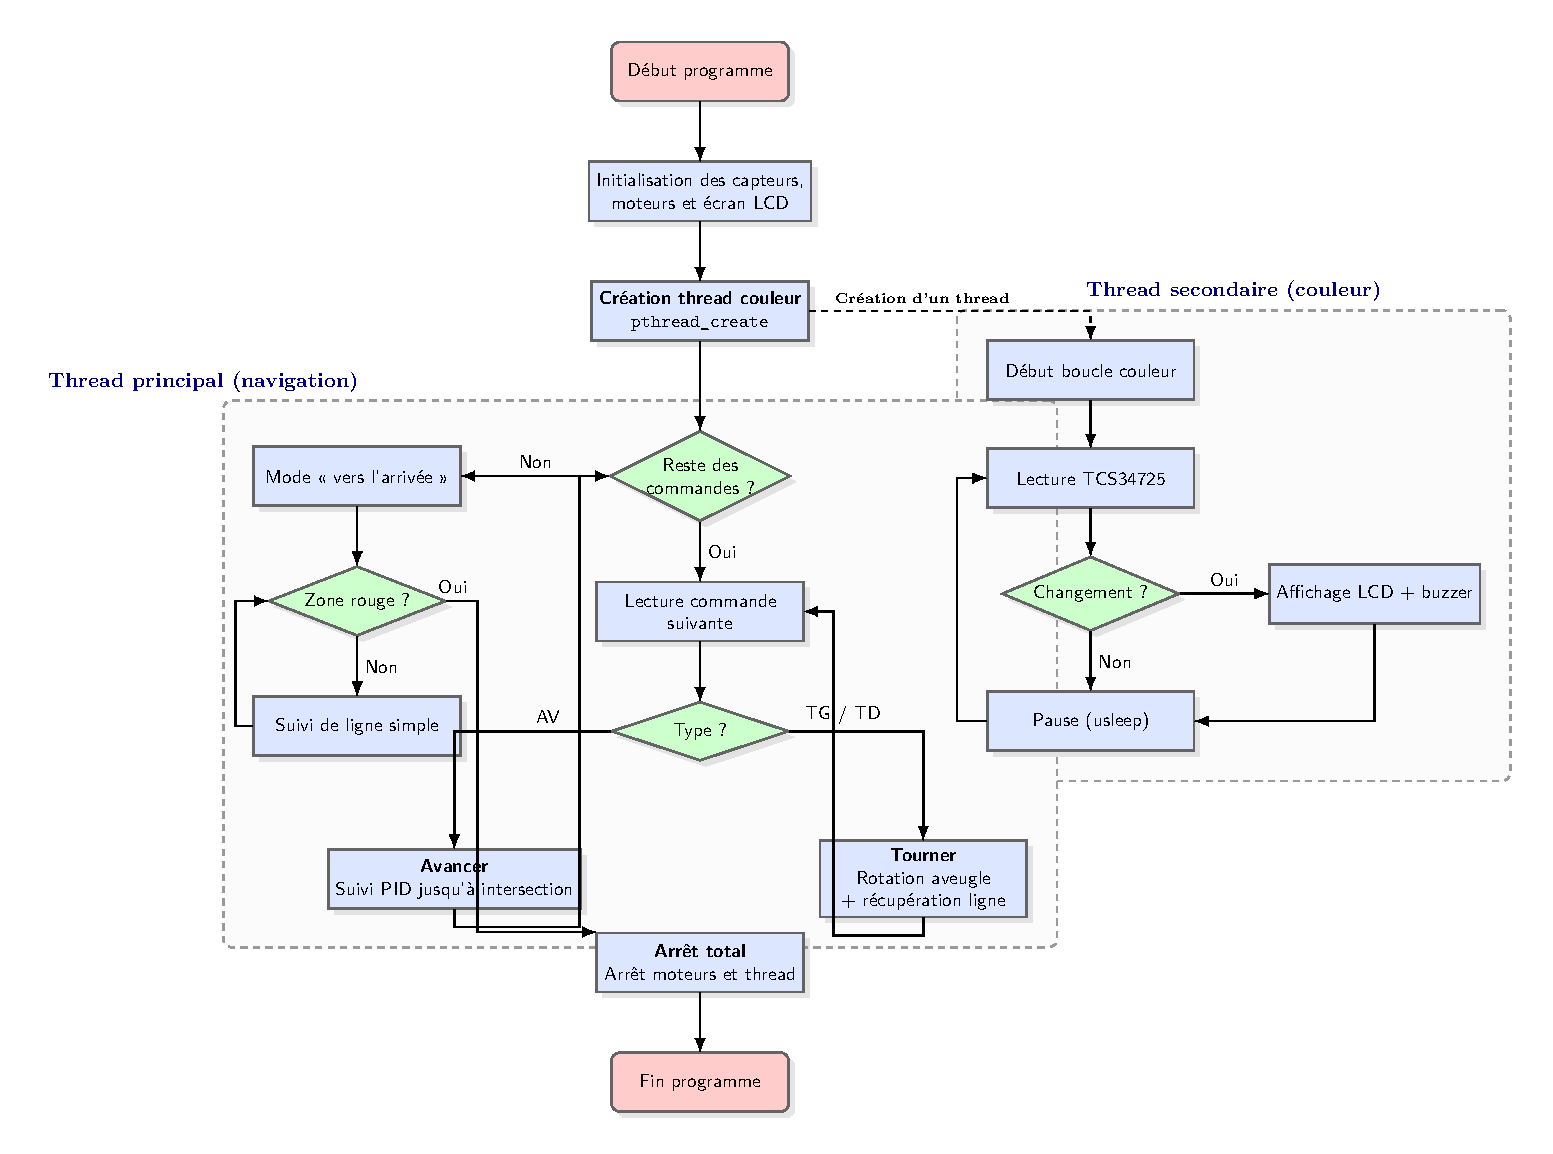
\includegraphics[height=16cm, keepaspectratio,angle=90]{images/flowchart.pdf}